\setchapterpreamble[u]{\margintoc}
\chapter{Energy Systems}
\labch{tut1}


After completing this session successfully, you should be able

\begin{itemize}
\item to understand what an energy system is,
\item to know about issues connected with current energy systems, and
\item to explain the necessity of energy system transitions.
\end{itemize}


\section{What is an energy system?}

\paragraph*{Defining energy and energy system.}

\begin{kaobox}[frametitle=Task]
What do you think about when you hear the word \textit{energy}? What do you think an \textit{energy system} is?
\end{kaobox}

\begin{definition}
\labdef{energy}
Energy is the capacity for doing work. It can exist in potential, kinetic, thermal, chemical, and various other forms \sidecite{britannica_the_editors_of_encyclopaedia_energy_nodate}.
\end{definition}

\begin{definition}
\labdef{es}
The energy system encompasses all components involved in the production, conversion, delivery, and use of energy \sidecite{intergovernmental_panel_on_climate_change_climate_2014}.
\end{definition}

It is important to have in mind that the whole purpose of the energy system is to fulfil the demand for energy services to satisfy human needs. Thus, the energy system is also sometimes defined as all arrangements whereby humans make use of the Earth’s energy resources to enhance their lives \sidecite{smil_energy_2010}.

% TODO: add a side note on what energy resources are (including fossil, renewable examples, etc.)

\paragraph*{Understanding what is part of the energy system.}

\begin{kaobox}[frametitle=Task]
Look at the photos in \reffig{es_photos}, what do you think is part of the energy system? Can you identify different types of elements of the energy system?
\end{kaobox}

\begin{figure}[hb]
	\includegraphics[height=0.34\textwidth]{files/ES_photo_1.jpg}
	\includegraphics[height=0.34\textwidth]{files/ES_photo_2.jpg}\\
	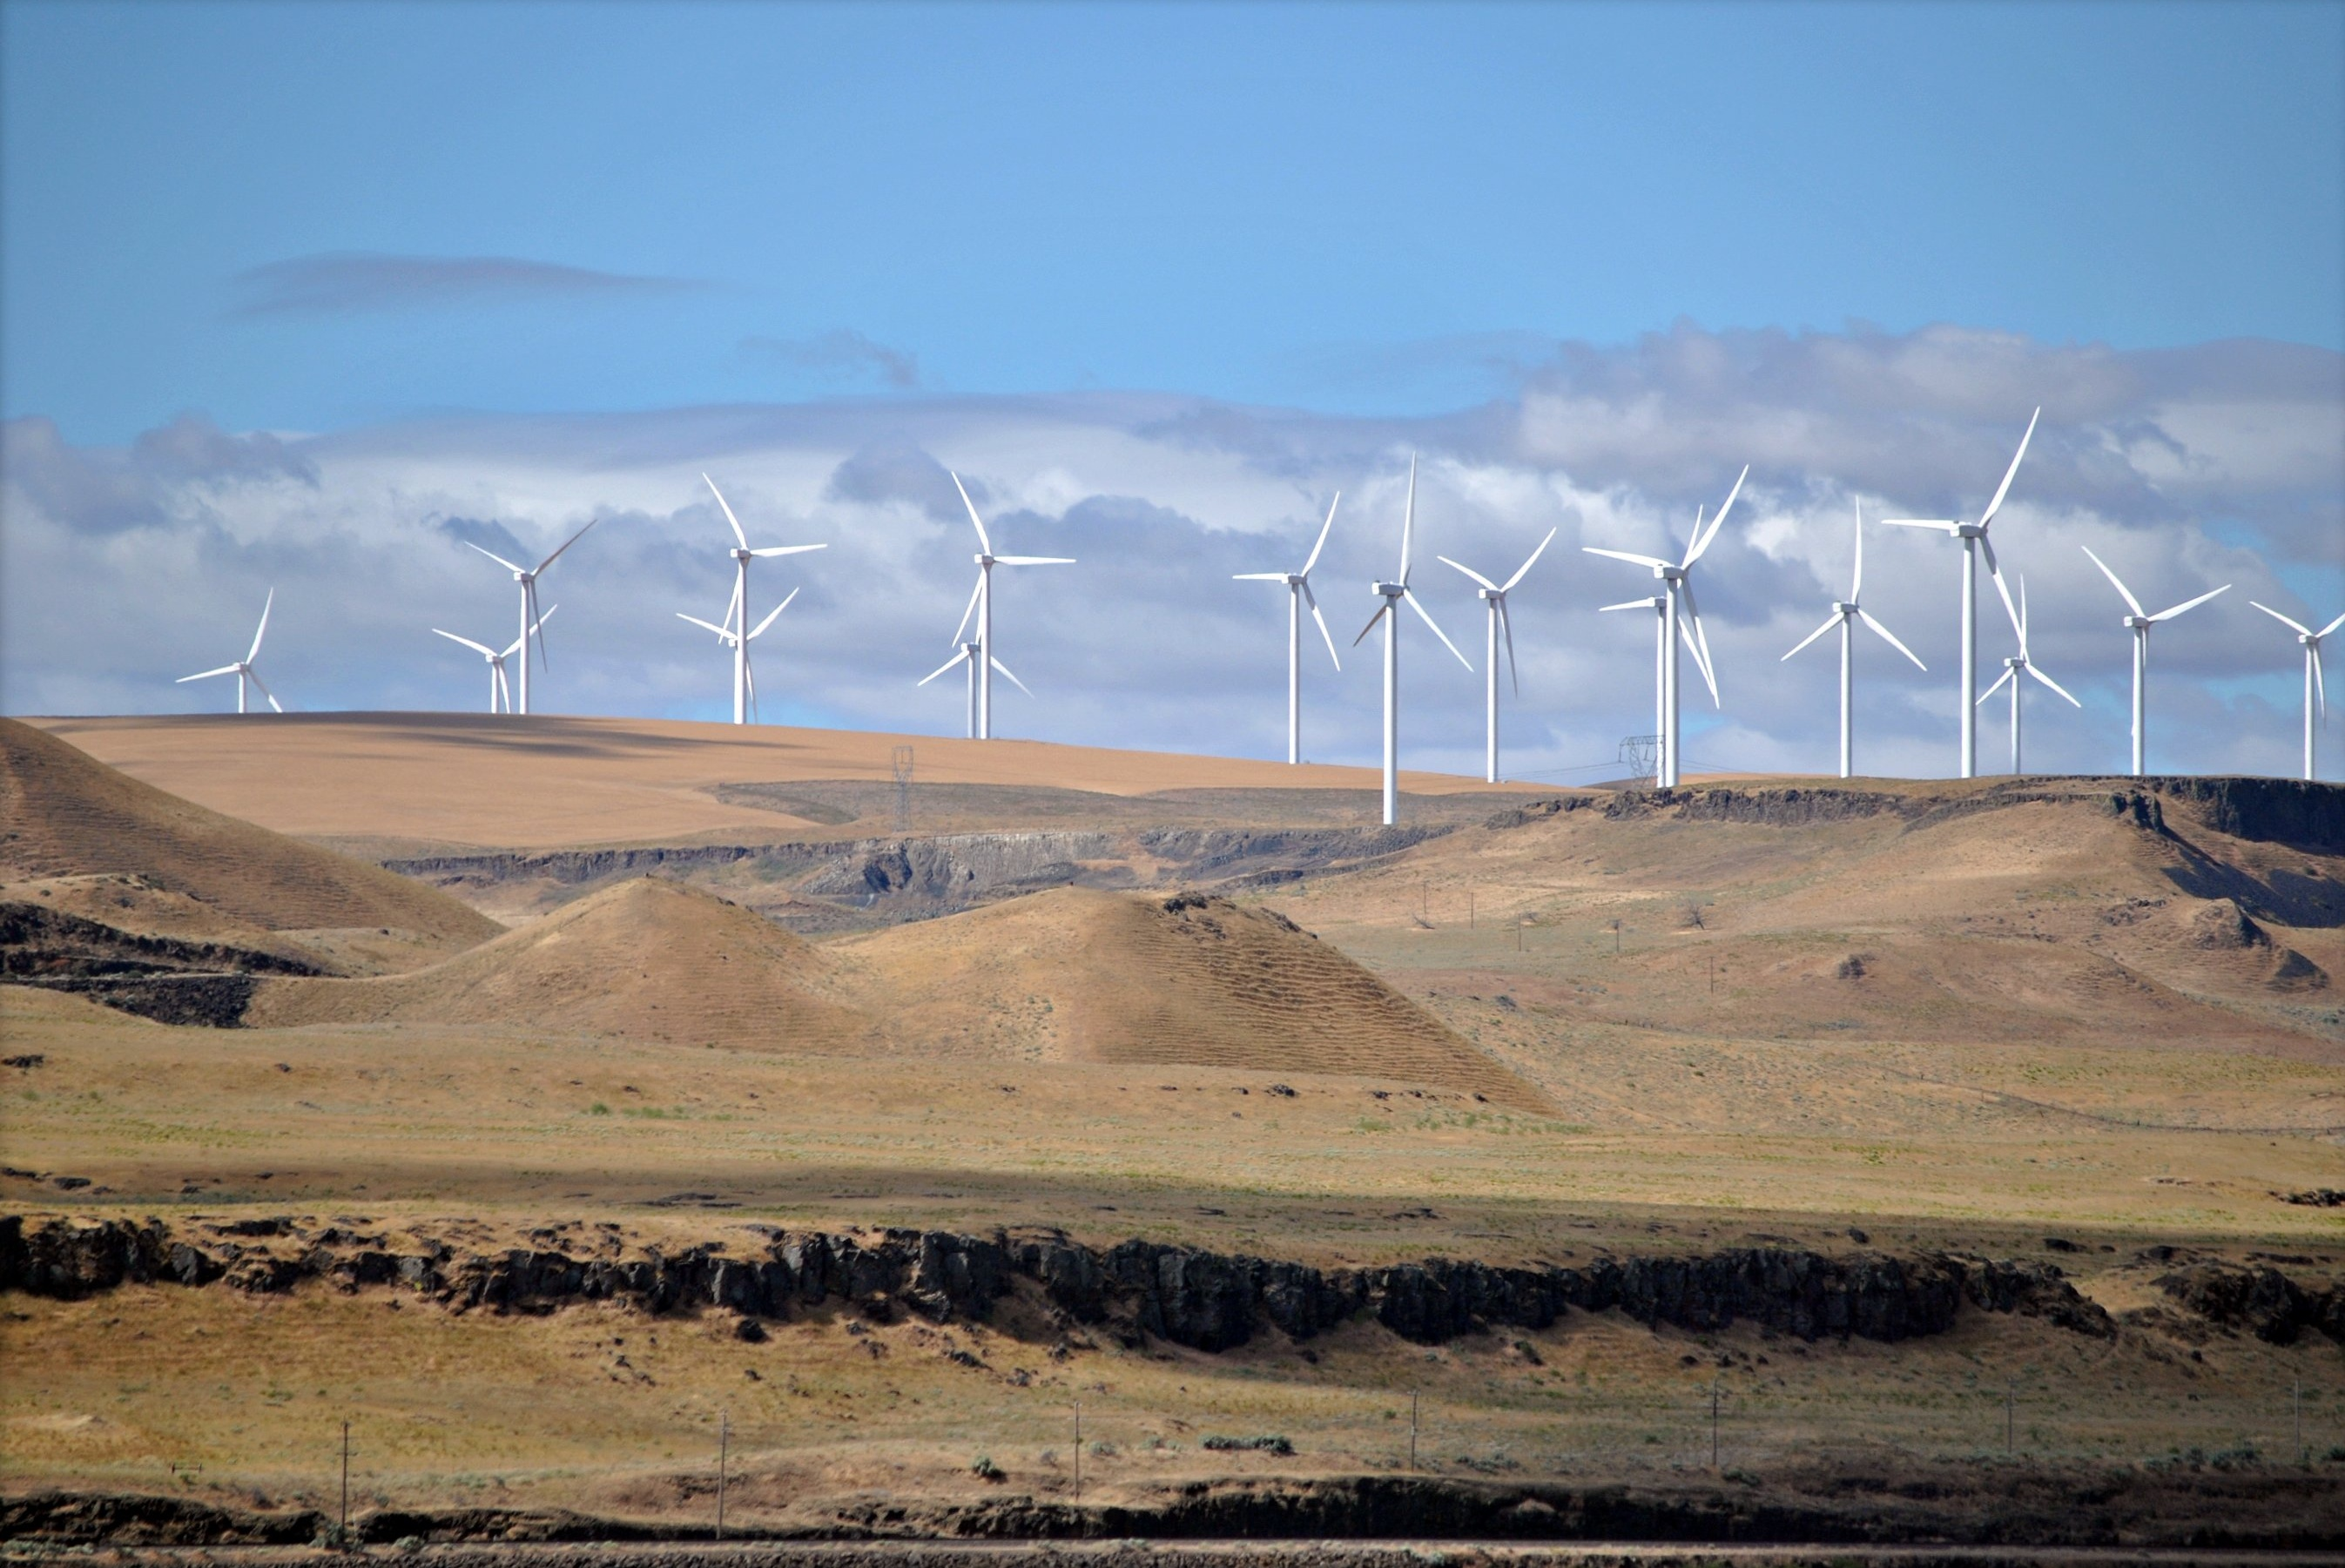
\includegraphics[height=0.34\textwidth]{files/ES_photo_3.jpg}
	\includegraphics[height=0.34\textwidth]{files/ES_photo_4.jpg}
	\caption[Photos showing different parts of the energy system.]{Photos showing different parts of the energy system. Bottom right photo, \copyright Leonhard Hofbauer, 2021, released under a CC-BY-4.0, the remaining photos, clockwise, are from Steve Wilson, VasenkaPhotography, and Stig Nygaard, respectively, and all licensed under a CC-BY-2.0.}
\labfig{es_photos}
\end{figure}


 
\section{Major issues of current energy systems}
\labsec{issues}

\paragraph*{Considering problems connected to current energy systems.}

\begin{kaobox}[frametitle= Excerpt from \sidecite{maciel_energy_2012} (reprinted under a CC-BY-4.0), backgroundcolor=Goldenrod!45!white,frametitlebackgroundcolor=Goldenrod!45!white]
Worldwide, transportation generates over 23\% of the total of greenhouse gas emissions arising from the use of energy and accounts for at least 26\% of the planet's energy consumption [1,2,3,4,5,6]. The transportation sector occupies between 15\% and 25\% of the land mass in major cities throughout the World [7,8,9,10,11], and the time lost in traffic congestion in several countries leads to an economic loss of approximately 1 to 3\% of GDP [12].\\

Furthermore, over a million people die and three million are injured every year in road traffic accidents worldwide [13,14,15]. These accidents result in economic costs of approximately 5\% of GDP in some countries [16]. Several countries considered to be `emerging' economically, such as Brazil, have adopted transportation systems that repeat the errors committed by more developed countries, including the encouragement of individual motorized transportation as the standard model. This has not proved to be the optimal solution [17].\\

Additionally, studies on the causes of persistent poverty in the peripheral areas of large cities, both in developed and emerging countries, point to a lack of transportation as one of the principal causes of social ills [18]. It is clear that an economy suffers significant losses in the absence of adequate transportation support. A sustainable transportation strategy has the potential to make a significant contribution to the environmental, economic and social development of cities and surrounding areas [19].\\

In Brazil, where the government regularly proclaims its overriding commitment to both the efficient use of public resources and the improvement of living standards for the population, there is an urgent and evident need for a drastic overhaul of the currently unsustainable transportation system. An accurate and reliable projection of the consumption of resources and the level of emissions produced by our transportation system in the coming decades is a key factor in ensuring the adequate redirection of public policies and the consequent benefits to the population.
\end{kaobox}

\begin{kaobox}[frametitle=Task]
Read through the box above, which talks about the transport sector, a part of the energy system. What issues related to the current transport system are mentioned? Are these issues also existing more widely in other parts of the energy system? Can you think of any other issues connected to the current transport and energy system not mentioned in the text?
\end{kaobox}

\section{The energy transition}

\paragraph*{The need for energy transitions.}~\\

% TODO: add a definition and/or more information on the energy transition in a side note

The issues discussed in the previous section -- climate change, pollution, health impacts, energy poverty, and others -- require that we change the way societies extract, transport, and use energy. This is often described as energy transition.

\begin{kaobox}[frametitle=Task]
Who do you think is responsible for the energy transition? Why?
\end{kaobox}


\section{Homework}
\labsec{hw1}

\begin{figure}[hb]
	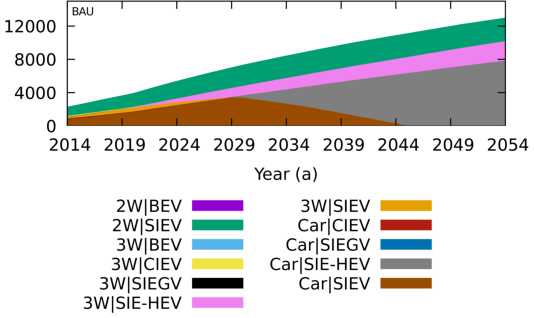
\includegraphics[width=0.95\textwidth]{files/india_transport.pdf}
	\caption[Transport sector pathway for India.]{Graph showing the passenger transport performance in billion person kilometres (bpkm) for a potential pathway for the Indian road transport system (2W: motorcycle, 3W: 3-wheeler motorcycle, BEV: battery electric vehicle, CIEV: diesel vehicle, FCV: fuel cell hydrogen vehicle, HEV: hybrid electric vehicle, SIEGV: CNG/gas vehicle, SIEV: petrol vehicle). Adopted from \cite{hofbauer_shaping_2018}.}
	\labfig{india_transport}
\end{figure}


\reffig{india_transport} above shows how the road transport sector in India might develop in future. It was part of a study that described several of those possible future pathways.

Write a text that covers the following three elements:
\begin{itemize}
\item Write a short description the development shown in the figure.
\item Research and discuss one or two social or environmental problems of the energy system in India at the moment and explain how this development could worsen or improve these problems.
\item Describe changes one could make to this development to solve these issues.
\end{itemize}


Please have the following points in mind when working on your assignment:

\begin{itemize}
\item Your assignment needs to be 500 $\pm$ 10\% words long.
\item You need to submit your assignment on the platform and before the deadline mentioned by your course leader.
\item If you have any questions while working on the assignment, do not hesitate to approach your course leader.
\end{itemize}